% !TeX root = ../../book.tex
\section{涉及集合的证明}

现在我们已经了解了许多定义和示例,为了介绍什么是集合以及如何操作它们,让我们实际写一些关于集合的严格的、数学上正确的、良好撰写的\textbf{证明}。这里包含的所有命题/引理都是有用的事实,我们可以稍后引用,并且我们希望你能够证明这些主张。(注:引理只是一个需要一些证明的小结果,稍后可以引用来证明更重要的定理。)此外,所有这些证明都具有将来期望你也能提供的质量和严谨性,不久的将来……如果你愿意,可以用此作为指导!

\subsection{逻辑且严谨:使用定义}

这里要强调的一点是,当我们从描述性的、``冗长的''和直观的证明过渡到更严格的、数学上正确的和正式撰写的证明时,\textbf{正规定义非常重要}。从根本上讲,它们是必不可少的,因为当我们说``$A \cup B$''时,我们需要知道你确切地知道该符号的含义以及它如何在集合 $A$ 和 $B$ 上运行。

另一个例子,当我们说``证明 $A = B$''时,我们心中有一个非常具体的目标,并且你需要跟我们保持一致。对主要概念有直观理解总是有帮助的---``哦,陈述 $A = B$ 只是意味着 $A$ 和 $B$ 具有相同的元素''---但这\emph{不是}我们想要在严格证明中使用的语言/想法。为了证明 $A = B$ 这样的命题,我们需要\textbf{诉诸}集合上下文中``$=$''的\textbf{定义}:$A = B$ 当且仅当 $A \subseteq B$ 且 $B \subseteq A$。

这就是我们说的``满足定义"或``诉诸定义"的含义:要证明某个数学对象具有某种属性,你必须证明该对象满足该属性的正式定义。如果你不熟悉该定义,或者忘记了如何准确地表述它……无论如何,都应该去了解它!我们知道到需要吸收大量新信息,并且当你对某事还不熟悉时,忘记某些地方也在所难免。通过这样做,你将开始更快、更牢固地消化吸收这些想法。

在下面的示例中,你将看到我们如何使用 ``$\subseteq$''、``$=$'' 和 ``$\cap$'' 等定义。对于每个命题/引理,我们最终都会撰写一个正式的证明,但我们也会写出如何\emph{提出这样一个证明}的内容。通常这才是困难的部分!我们认为你会注意到,其中许多解释只是回忆相关定义并思考它的含义以及它在给定情况下应该如何应用。某种程度上,这就是数学。我们只是让我们使用的定义变得越来越复杂。

\subsection{证明 ``$\subseteq$''}

回想一下子集的定义,因为接下来我们会频繁使用它:

\begin{definition}
    给定两个集合 $A$ 和 $B$,如果 $A$ 的每个元素也是 $B$ 的元素,那么我们说 $A$ 是 $B$ 的\dotuline{子集}。
\end{definition}

假设我们遇到如下问题:
\begin{center}
    设 $A$ 为集合…… 并设 $B$ 为集合…… 证明 $A \subseteq B$。
\end{center}
我们如何利用 $A \subseteq B$ 的定义来证明这个主张?是的,直观的想法是``$A$ 的每个元素也是 $B$ 的元素'',但我们不应该只是试图绕过这个问题而将这句话作为我们的结论。相反,我们需要验证 $A$ 的每个元素也必然是 $B$ 的元素。这就是``\textbf{任意固定}'' 这句美妙的短语派上用场的地方!

\subsubsection*{``任意固定''}

我们怎样才能同时讨论 $A$ 的\emph{所有可能元素}呢?当然,如果 $A$ 只有 $3$ 个元素,我们可能只需一一检查即可。但是如果 $A$ 有 $100$ 个元素怎么办?如果有 $100$ 万个元素呢?甚至\emph{无穷}多个呢?我们怎样才能以合理的方式同时证明所有这些元素呢?

我们要做的就是引入 $A$ 的\textbf{任意固定}元素,这样我们就有了可以使用的东西。这个元素是\textbf{任意的},因为我们不对它是什么或它具有什么属性做任何额外的假设,只要它是 $A$ 的元素即可。这个元素是\textbf{固定的},因为我们将为其分配某个变量名(通常是一个字母,例如 $a$ 或 $x$ 或 $t$ 等),并且该字母在我们证明的其余部分中代表\emph{相同的}对象。只要我们能证明这个元素满足目标,那么我们就同时证明了 $A$ 的\emph{所有}元素。

\subsubsection*{示例}

让我们看看这个过程的实际应用,以真正理解这一点。我们将从要证明的陈述开始,接着描述提出证明的思维过程,然后给出正式的书面证明。

\begin{lemma}\label{lemma3.9.1}
    设 $A,B,X$ 为任意集合。如果 $X \subseteq A$ 且 $X \subseteq B$, 则 $X \subseteq A \cap B$。
\end{lemma}

\emph{直觉}:考虑绘制维恩(Venn)图来表示这种情况。为了确保 $X \subseteq A$ 和 $X \subseteq B$ 同时成立,我们需要令集合 $X$ 位于 $A$ 和 $B$ 的``内部''。相应地,这意味着 $X$ 必须完全位于 $A$ 和 $B$ 重叠的``内部'',即 $A \cap B$ 代表的部分。这有助于我们认识到这个说法确实是正确的。但这并不构成证明!
\begin{center}
    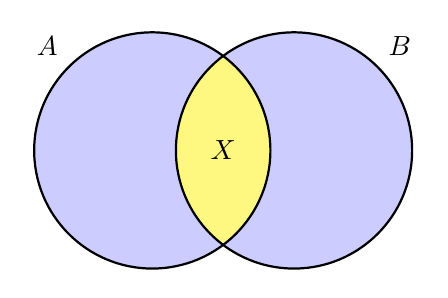
\begin{tikzpicture}[thick, set/.style = {circle, minimum size = 3cm, fill=blue!20}]

        % Set A
        \node[set,label={135:$A$}] (A) at (0,0) {};

        % Set B
        \node[set,label={45:$B$}] (B) at (1.8,0) {};

        % Intersection
        \begin{scope}
            \clip (0,0) circle(1.5cm);
            \clip (1.8,0) circle(1.5cm);
            \fill[yellow!50](0,0) circle(1.5cm);
        \end{scope}

        % Circles outline
        \draw (0,0) circle(1.5cm);
        \draw (1.8,0) circle(1.5cm);

        % Set intersection label
        \node at (0.9,0) {$X$};
    \end{tikzpicture} 
\end{center}

为了\emph{证明}这个命题,我们将引入任意固定的元素 $x \in X$。我们对它了解多少呢?我们假设 $X \subseteq A$。``$\subseteq$'' 的定义意味着 $X$ 的所有元素也是 $A$ 的元素。现在我们知道 $x$ 是 $X$ 的元素;这意味着它也是 $A$ 的一个元素。多么方便啊!我们可以对 $x$ 和 $X$ 和 $B$ 做出一些类似的陈述,这将告诉我们 $x \in B$。综上,这意味着什么?我们发现可以用 ``$\cap$'' 的定义,这告诉我们 $x \in A \cap B$。太棒了!现在,我们把它写下来。

\begin{proof}
    设 $x \in X$ 为任意固定元素。

    假设 $X \subseteq A$,根据 $\subseteq$ 的定义,可得 $x \in A$。

    同理,假设 $X \subseteq B$,可得 $x \in B$。

    因为 $x \in A$ 且 $x \in B$,根据 $\cap$ 的定义,这意味着 $x \in A \cap B$。

    综上,我们证明了当 $x \in X$ 时,$x \in A \cap B$ 也成立。由于 $x \in X$ 是任意的,因此我们得出 $X \subseteq A \cap B$ 的结论。
\end{proof}

怎么样,还不错吧?让我们看一个稍微复杂一点的例子。

\begin{proposition}
    设 $A$ 和 $B$ 为任意集合。则 $\mathcal{P}(A) \cap \mathcal{P}(B) \subseteq \mathcal{P}(A \cap B)$。
\end{proposition}

哇,这是真的吗? 回顾 \ref{sec:section3.5} 节中的问题 \ref{exc:exercises3.5.6},你会看到一个具体例子。这表明,\emph{一般而言},这一说法是正确的,而不仅仅是针对该示例。让我们找出为什么这是正确的,并证明它。

\emph{直觉}:这里有几个层次的定义共同发挥作用。特别是,幂集运算可能会让你感到困惑。关键是记住这个定义:$\mathcal{P}(A)$ 是 $A$ 的所有子集的集合。现在,这里的主要主张是一个子集关系:无论集合 $\mathcal{P}(A) \cap \mathcal{P}(B)$ 是什么(我们稍后会对其进行分析,但眼下重要的是你要立即意识到到它是什么类型的对象:集合),它应该是集合 $\mathcal{P}(A \cap B)$ 的子集。值得注意的是,这确实激发了即将到来的证明的总体形式。

甚至无需考虑 $\mathcal{P}(A) \cap \mathcal{P}(B)$ 的含义,我们就可以确定我们的证明将从``令 $X \in \mathcal{P}(A) \cap \mathcal{P}(B)$ 为任意固定集合''开始。这是因为我们需要通过获取左侧集合中的任意元素并推断它也是右侧集合中的元素来满足``$\subseteq$''的定义。这就是我们所说的证明的\textbf{结构}。

元素 $X \in \mathcal{P}(A) \cap \mathcal{P}(B)$ ``看起来像什么''?它是一个集合,并且是 $P(A)$ 和 $P(B)$ 的元素。这意味着……好吧,实际上我们现在要直接跳到正式证明,因为无论如何我们都会发现自己在下面重复相同的单词。但在继续阅读我们的证明之前,我们认为你应该尝试编写自己的证明。做完之后,你可以对比一下,看看你的做法是否正确,是不是和我们的步骤一样,写的是否清楚等等。看看你能做到什么程度!

\begin{proof}
    设 $X \in \mathcal{P}(A) \cap \mathcal{P}(B)$ 为任意固定集合。

    根据 $\cap$ 的定义,这意味着 $X \in \mathcal{P}(A)$ 且 $X \in \mathcal{P}(B)$。

    因为 $X \in \mathcal{P}(A)$,根据幂集的定义,我们知道 $X \subseteq A$。

    同理,因为 $X \in \mathcal{P}(B)$,我们知道 $X \subseteq B$。

    因为 $X \subseteq A$ 且 $X \subseteq B$,根据我们刚刚证明的引理 \ref{lemma3.9.1},可得 $X \subseteq A \cap B$。

    因为 $X \subseteq A \cap B$,根据幂集的定义,我们知道 $X \in \mathcal{P}(A \cap B)$。

    因为 $X$ 是任意固定集合,因此我们得出结论 $\mathcal{P}(A) \cap \mathcal{P}(B) \subseteq \mathcal{P}(A \cap B)$。
\end{proof}

你的证法跟上面的一样吗?你也引用了前面的引理吗?你是否在没有意识到的情况下再次证明了这个结果?把它当作一个教训!证明结果的主要好处之一是我们可以在以后的证明中使用它们!在一个证明过程中再次证明之前的结果在技术上并没有什么问题;但不重复证明会节省一点时间。如果你发现自己正在解决一个问题并发觉:“嘿,这感觉很熟悉……”,回去寻找相关的定理或引理或例子。也许你可以利用一些已经获得的知识来发挥自己的优势。

\subsection{证明 ``$=$''}

\subsubsection*{双重包含证明}

我们需要再一次回顾 ``$=$'' (在集合上下文中)的定义,因为我们将在这里频繁地使用它。

\begin{definition}
    我们说两个集合 $A$ 和 $B$ 相等,并写为 $A = B$,当且仅当 $A \subseteq B$ 且 $B \subseteq A$。
\end{definition}

就是这样!它完全是根据之前的定义 ``$\subseteq$'' 构建的(因为 ``$\supseteq$'' 的定义是完全等价的)。因此,这本身并不是一项新技术,因为它实际上是先前技术的重复应用。也就是说,要证明 $A = B$,我们只需使用上一小节中使用的技术,证明 $A \subseteq B$,然后证明 $B \subseteq A$。

事实上,这项技术非常常见,以至于被赋予了一个名字:\textbf{双重包含}。当我们以两种方式证明两个集合是彼此的子集并得出它们相等的结论时,我们将其称为\textbf{双重包含证明}。

\subsubsection*{示例}

让我们看一下双重包含技术的实际应用案例。

\begin{lemma}
    设 $A$ 和 $B$ 为任意集合。则 $A - (A \cap B) = A - B$。
\end{lemma}

\emph{直觉}:像往常一样,我们可以画一个维恩图来说服自己相信这一事实,但这并不能证明任何事情。相反,我们将采用双重包含证明。如果我们取一个元素 $x \in A - (A \cap B)$,我们可以先应用 ``$-$'' 的定义,然后应用 ``$\cap$'' 的定义,来推导出有关 $x$ 的信息。希望能够得到 $x \in A - B$。然后,如果我们取一个元素 $y \in A - B$,希望我们可以应用一些定义来推断出 $y \in A - (A \cap B)$。 也许我们还不确定具体如何做到这一点,但通过查看维恩图并使用定义,我们肯定可以弄清楚。你为什么不先尝试一下,然后再阅读我们的证明!

\begin{proof}
    我们将采用双重包含证明来证明 $A - (A \cap B) = A - B$。

    (``$\subseteq$'')首先,设 $x \in A - (A \cap B)$ 为任意固定元素。根据 ``$-$'' 的定义,我们知道 $x \in A$ 但 $x \notin A \cap B$。这意味着 $x$ 既是 $A$ 的元素又是 $B$ 的元素\emph{不}可能成立。我们已知 $x \in A$, 那么可以推导出 $x \notin B$。因此,$x \in A$ 且 $x \notin B$。根据 ``$-$'' 的定义,可以推导出 $x \in A-B$。这就证明了 $A - (A \cap B) \subseteq A - B$。


    (``$\supseteq$'')接着,设 $y \in A - B$ 为任意固定元素。根据 ``$-$'' 的定义,这意味着 $y \in A$ 且 $y \notin B$。因为 $y$ 不是 $B$ 的元素,这意味着 $y$ 当然不可能同时是 $A$ 和 $B$ 的元素。根据 ``$\cap$'' 的定义,即 $y \notin A \cap B$。因为我们知道 $y \in A$ 且 $y \notin A \cap B$,我们可以推导出 $y \in A - (A \cap B)$。这就证明了 $A - B \subseteq A - (A \cap B)$。

    综上,利用双重包含证明,我们证明出 $A - (A \cap B) = A - B$。
\end{proof}

纵观上面证明的整体结构。我们看到它分为两部分,因为它是一个双重包含证明,我们\emph{很友善地提前}向勇敢的读者指出了这一点,并将这两个部分适当地分开。从技术上讲,忽略这一点并直接深入证明也是正确的,但这可能会让读者感到困惑。证明的全部意义在于\emph{让别人信服}你已经弄清楚的事实,所以最好让他们尽可能容易地理解你正在做的事情。

让我们再看另一个证明两个集合相等的例子。这个例子会有点不同,因为双重包含的一部分将利用补集操作。作为预览,现在花一点时间思考为什么陈述 $A \subseteq B$ 和 $\overline{B} \subseteq \overline{A}$ 是\emph{等价的}(假设存在某个全集 $U$,满足 $A, B \subseteq U$)。画出维恩图并尝试举一些例子。甚至尝试证明这一点!

\begin{proposition}
    \[\Big\{x \in \mathbb{N} \mid x + \frac{8}{x} \le 6\Big\} = \{2, 3, 4\}\]
\end{proposition}

\begin{proof}
    设 $A = \Big\{x \in \mathbb{N} \mid x + \frac{8}{x} \le 6\Big\}, B = \{2, 3, 4\}$,要证明 $A = B$,我们需要证明 $A \subseteq B$ 且 $B \subseteq A$。

    首先证明 $B \subseteq A$。我们可以分别考虑这三个元素,并验证它们是否满足 A 的定义不等式:
    \begin{align*}
        2 + \frac{8}{2} &= 6 \le 6 \\
        3 + \frac{8}{3} &= \frac{17}{3} \le 6 \\
        4 + \frac{8}{4} &= 6 \le 6
    \end{align*}
    因为 $2,3,4 \in \mathbb{N}$,我们推导出 $2 \in A, 3 \in A, 4 \in A$,所以 $B \subseteq A$。

    接着证明 $A \subset B$。我们将证明 $\overline{B} \subseteq \overline{A}$,其中补集是在 $\mathbb{N}$ 作为全集的情况中获取的。也就是说,我们将证明所有自然数 $1,5,6,7,\dots$ \emph{不是} $A$ 的元素。

    为了证明这一点,我们将验证这些元素中的任何一个都\emph{不}满足 $A$ 的不等式定义。

    前两个情况很容易验证:$1 + \frac{8}{1} = 9 \nleq 6$ 且 $5 + \frac{8}{5} = \frac{33}{5} \nleq 6$。

    对于其他情况,我们可以取任意固定元素 $x \in \mathbb{N}$ 且 $x \ge 6$,此时不等式可以写为 $x + \frac{8}{x} \ge 6 + \frac{8}{x}$,因为 $\frac{8}{x} > 0$,所以 $x + \frac{8}{x} \ge 6 + \frac{8}{x} > 6$。

    这表明只有 $2,3,4$ 满足 $A$ 的不等式定义。

    综上,利用双重包含证明,我们证明出 $A = B$。
\end{proof}

仔细思考一下为什么证明后半部分采用的方法是有效的。(这实际上是条件陈述的\textbf{逆否}形式的一个实例,但我们还没有定义这些术语;我们将在下一章讨论逻辑时详细讲述。)

让我们看另一个证明集合相等的例子。这个略有不同,因为我们要证明某个集合实际上是空集,为此,我们将证明它没有元素。

\begin{proposition}
    对于每个 $n \in \mathbb{N}$,定义 $S_n = \mathbb{N}-[n]$。那么
    \[\bigcap_{n \in \mathbb{N}}S_n = \varnothing\]
\end{proposition}

如果你不理解上面式子的含义,建议你尝试几个例子。比如,看一下集合 $S_1, S_1 \cap S_2, S_1 \cap S_2 \cap S_3$ 的元素,依此类推。先尝试找出左侧大交集的候选元素,然后找出为什么它实际上不是该集合的元素。之后,尝试找出一种正式的证明并写出来; 看看下面我们是怎么做的吧!

\begin{proof}
    设 $T = \bigcap_{n \in \mathbb{N}}S_n$,便于我们后面引用它。

    要证明 $T = \varnothing$,我们需要证明 $T$ 中没有任何元素。请注意,$T$ 由许多自然数集合的交集形成,因此很明显,$T$ 中元素只可能是自然数。

    考虑任意固定元素 $x \in \mathbb{N}$,我们需要证明 $x \notin T$。

    我们知道 $x \in [x] = \{1,2,\dots, X\}$,因此根据 ``$-$'' 的定义,$x \notin \mathbb{N}-[x]$。

    根据定义,$T$ 包含属于 $\mathbb{N} - [n]$ 形式的所有集合的元素。我们已经(至少)确定了交集中的一个集合 $\mathbb{N} - [x]$,使得 $x$ 不属于该集合。因此,$x$ 不可能是 $T$ 的元素,因为它不属于所有此类集合,所以 $x \notin T$。

    因为 $x \in \mathbb{N}$ 是任意的,我们证明了 $T$ 的元素中不包含自然数,因此它根本没有元素。
\end{proof}

\emph{总结}:让我们再说明一下这项技术为何有效。我们证明 $T$ 中没有元素,即 $T \subseteq \varnothing$。这就完成了整个过程,因为 $\varnothing \subseteq T$ 无需证明,它对于任何集合都成立。因此,双重包含论证的一部分已经实现,我们可以得出 $T = \varnothing$ 的结论。

让我们再举一个例子。我们希望引入这个例子,是因为它为我们提供了使用索引集操作的进一步练习。在本节的练习中你会发现许多类似的问题。我们鼓励你尽可能多地参与其中!

\begin{proposition}
    对于每个 $n \in \mathbb{N}$,定义 $A_n = \{x \in \mathbb{R} \mid 0 \le x < \frac{1}{n}\}$。那么
    \[\bigcap_{n \in \mathbb{N}}A_n = \{0\}\]
\end{proposition}

想想这上面命题意味着什么。在数轴上画出 $A_n$ 集合的图。``$\cap$'' 有什么作用?为什么会得出 $0$ 是该交集的元素?为什么它是\emph{唯一的}元素?

``$\cap$'' 的定义在这个证明中至关重要,所以让我们回顾一下这里的定义。这里的关键词是\emph{对于每个}:

\begin{definition}
    由集合 $I$ 索引的一系列集合 $A_i$ 的交集为
    \[\bigcap_{i \in I} A_i = \{x \in U \mid x \in A_i \;\text{对于每个}\; i \in I\}\]
    其中我们假设存在集合 $U$ 满足对于每个 $i \in I, A_i \subseteq U$。
\end{definition}

也就是说,请记住,多个集合的索引交集将属于所有组成集合的元素聚合在一起。因此,在下面的证明中,你将看到我们需要证明
\begin{enumerate}[label=(\arabic*)]
    \item $0$ 确实是所有 $A_n$ 集合的元素。
    \item 没有其他数字是所有集合的元素,即对于每个非零实数,我们可以找到至少一个 $A_n$ 集合,使得该数字不是该集合的元素。
\end{enumerate} 

\begin{proof}
    首先,我们来证明
    \[\{0\} \subseteq \bigcap_{n \in \mathbb{N}}A_n\]
    这需要我们证明对于每个 $n \in \mathbb{N}, 0 \in A_n$。

    设 $n \in \mathbb{N}$ 为任意固定元素。注意,不等式 $0 \le 0 \le \frac{1}{n}$ 必然成立。

    (注:你可能会担心,因为``在极限内'' $0$ 不会``同时''小于每个分数 $\frac{1}{n}$,但这不是重点!正确的思路是:$0 \in A_1$ 吗?是的,因为 $0 \le 0 < 1$。$0 \in A_2$ 吗?是的,因为 $0 \le 0 < \frac{1}{2}$。$0 \in A_3$ 吗?是的,因为 $0 \le 0 < \frac{1}{3}$。依此类推。该不等式对于每个 $n \in N$ 分别成立,所以 $0$ 是每个此类集合的元素。如果你不担心这一点,没关系!继续前进!)

    因此,对于每个 $n \in \mathbb{N}, 0 \in A_n$,所以根据 ``$\cap$'' 的定义 $\displaystyle{0 \in \bigcap_{n \in \mathbb{N}} A_n}$。这就证明了 $\displaystyle{\{0\} \subseteq \bigcap_{n \in \mathbb{N}} A_n}$。

    接着,我们来证明
    \[\bigcap_{n \in \mathbb{N}}A_n \subseteq \{0\}\]
    我们将通过设 $\mathbb{R}$ 为全集的情况下考虑这些集合的\emph{补集}来做到这一点。具体来说,我们将证明
    \[\overline{\{0\}} \subseteq \overline{\bigcap_{n \in \mathbb{N}}A_n}\]
    这意味着我们要证明每个非零实数\emph{不是每个} $A_n$ 的元素。

    设 $x \in \mathbb{R}$ 为任意固定元素,且 $x \ne 0$。也就是说,要么 $x > 0$ 要么 $x < 0$。我们加下来将分这两种情况讨论。

    \emph{情况 1}:假设 $x > 0$。考虑实数 $\frac{1}{x} \in \mathbb{R}$。由于 $\mathbb{R}$ 中的自然数是无限且无界的,因此我们可以选择一个\emph{大于}该实数的自然数 $M$。也就是说,我们可以选择 $M \in \mathbb{N}$ 使得 $M > \frac{1}{x}$。

    (注意:想想为什么会这样。我们还没有\emph{证明} $\mathbb{N}$ 是无限的,或者数字沿着 $\mathbb{R}$ 的数轴``永远延续下去'',但我们希望这些想法对你来说直观且合理。)

    取 $M \in \mathbb{N}$ 且 $M > \frac{1}{x}$。由于 $x > 0$,我们可以将不等式两边同时乘以 $x$;由于 $M > 0$(因此 $\frac{1}{M} > 0$),我们可以再次乘以 $\frac{1}{M}$。由此得到 $x > \frac{1}{M}$。相应地,$x \ne A_M$,因为 $-\frac{1}{M} < x < \frac{1}{M}$ 为假。

    由于 $x \notin A_M$,所以 $x$ 肯定不是所有此类集合的元素。因此 $\displaystyle{x \notin \bigcap_{n \in \mathbb{N}} A_n}$

    \emph{情况 2}:假设 $x < 0$。我们采用跟前面类似的论证;这次,我们只考虑 $-x$,因为 $-x > 0$。使用与上面相同的逻辑,我们肯定可以找到满足 $M > \frac{1}{-x} = -\frac{1}{x}$ 的自然数 $M \in \mathbb{N}$。整理不等式可得 $x < -\frac{1}{M}$。因此 $x \notin A_M$,所以 $\displaystyle{x \notin \bigcap_{n \in \mathbb{N}} A_n}$。

    综上,我们已经证明,任意 $x \in \mathbb{R}$ 且 $x \ne 0$ 都不是至少一个 $A_n$ 集合的元素,因此任何这样的 $x$ 都不是它们交集的元素。因此,$\displaystyle{{0} \subseteq \bigcap_{n \in \mathbb{N}} A_n}$,并且我们已经通过双重包含论证证明了该主张。
\end{proof}

这个证明比其他证明更难一些,所以请务必多阅读几次,确保你理解每个步骤的思路和内容。特别是,考虑一下我们是如何选择 $M \in \mathbb{N}$ 满足 $M > \frac{1}{x}$ 这一步的步骤。你认为我们神奇地凭直觉做出了这个选择吗?或者我们是否认识到我们希望 $x < \frac{1}{M}$ 对于某些 $M$ 成立,进一步整理不等式以找出如何实现这一点?

\subsection{证伪}

\subsubsection*{举个例子}

考虑如下命题:
\begin{center}
    对于任意集合 $F, G, H$,如果 $F \subseteq G \cup H$,则要么 $F \subseteq G$ 要么 $F \subseteq H$。
\end{center}

这种说法成立吗?如果成立,我们该如何证明呢?我们取任意固定元素 $x \in F$。由于 $F \subseteq G \cup H$,这告诉我们 $x \in G \cup H$。 相应地,$x \in G$ 或 $x \in H$。这都没错吧?我们的证明完成了吗?

我们希望你能看出来这是行不通的!特别是,我们最后还没有满足 ``$\subseteq$'' 的定义。如果我们的目标是证明 ``$F \subseteq G$ 或 $F \subseteq H$'',那么我们应该得出结论,其中一个或另一个成立:即 $F$ 的\emph{每个}元素都是 $G$ 的元素,或者 $F$ 的\emph{每个}元素都是 $H$ 的元素。

我们发现 $F$ 的每个元素本身要么是 $G$ 的元素,要么是 $H$ 的元素,但我们不能确定 $F$ 的所有元素都是 $G$ 的元素或都是 $H$ 的元素。再次通读最后两段,以确保你跟上了逻辑。可能很容易为这个命题写出一个``证据'',却没有意识到你迈出了错误的一步!

\subsubsection*{定位错误}

这种对错误的识别是我们要发展的技能之一,它将在多个方面提供帮助。你会注意到,许多练习(到目前为止有一些,但随着我们继续深入,会有更多)要求你找出某些主张``证明''中的缺陷。通过指出存在缺陷,从而帮助你获得正确的证明(或多个证明,视情况而定)。阅读在逻辑、事实和清晰度上有误的证明是一项基本技能。更重要的是,仔细阅读别人的成果必然会让你成为一个对自己的成果更加挑剔的读者,并且会帮助你发现像前面段落中那样的潜在错误。如果你没有抓住它,请不要担心;既然你已经看到了它,你将来就会留意类似的错误!正如我们所说,这项技能是不断发展起来的,到读完本书时,你将成为数学证明的出色读者和作者。

\subsubsection*{反例}

那么,现在我们该怎么办?我们刚刚意识到我们上面的``证明''不起作用。这是否意味着该说法实际上是错误的?实际上,这一切意味着(到目前为止)我们的证明尝试失败了。也许其他一些逻辑路线会神奇地把我们带到难以捉摸的结论。

或者,也许这个说法确实是错误的。我们怎样才能证明这一点?考虑一下该命题的逻辑形式:它说某些陈述对于任意集合 $F,G,H$ 都成立。它说假设 $F \subseteq G \cup H$ 总是必然意味着 $F \subseteq G$ 或 $F \subseteq H$。要证明这并不总是成立,我们只需要找到所谓的\textbf{反例}即可。

我们将在下一章形式化逻辑时再次讨论所有这些想法,但现在你需要知道的是:\textbf{反例}是一个具体的、详细的、描述性的例子,它说明了关于``每个……''或``任意……''或``皆可能……''实际上并\emph{不}适用于所有情况。反例相当于通过展示该类中\emph{不具有}该属性的一个对象来\textbf{反驳}整个类对象具有某种属性的陈述。

\subsubsection*{示例}

让我们看一下寻找和陈述反例的过程如何解决我们上面的例子。

\begin{example}
    对于任意集合 $F, G, H$,如果 $F \subseteq G \cup H$,则要么 $F \subseteq G$ 要么 $F \subseteq H$。
\end{example}

这个命题应该适用于任意集合 $F,G,H$,因此当我们描述反例时,我们最好\emph{准确地}描述这三个集合是什么。我们不能只是解释解决这个问题的方法并讨论如何可能存在具有特定属性的三个集合。我们必须通过明确定义它们来告诉读者它们到底是什么。这就是我们反驳这一主张的第一行,但我们不能直接跳到这一点,因为我们还不知道如何定义它们!

这就是工作或乐趣所在:我们需要尝试这些集合所需的属性来帮助我们想出一个例子。回想一下,我们希望这些集合满足某些属性:我们应该确保假设 $F \subseteq G \cup H$ 成立,但我们希望结论 --- $F \subseteq G$ 或 $F \subseteq H$ --- 为假。

这是意味着什么呢?好吧,我们认为你会同意,从逻辑上讲,该陈述的``相反''或``否定''是 ``$F \not\subseteq G$'' 和 ``$F \not\subseteq H$''。(\textbf{逻辑否定}的概念将在下一章中再次出现;目前,我们认为你可以通过应用指导日常生活的逻辑原则来理解它。很快,我们将正式化这一想法。)

我们现在有一个具体的目标:找到满足以下所有三个条件的三个集合 $F,G,H$:

\begin{align*}
    F &\subseteq G \cup H \\
    F &\not\subseteq G \\
    F &\not\subseteq H \\
\end{align*}

接下来需要考虑的一件事是 ``$\not\subseteq$'' 的含义。我们有 ``$\subseteq$'' 的定义,那么它的``相反''或``否定''是什么?为了使 $F \subseteq G$ 成立,我们要求 $F$ 的每个元素也是 $G$ 的元素;因此,如果不成立,那么 $F$ 中至少有一个元素不是 $G$ 的元素。同理也适用于 $F \not\subseteq H$。现在,我们可以通过应用定义以一种有用的方式重申我们的目标:

\begin{align*}
    &F \text{的每个元素都是} G \text{的元素或} H \text{的元素} \\
    &F \text{中至少有一个元素不是} G \text{的元素} \\
    &F \text{中至少有一个元素不是} H \text{的元素} \\
\end{align*}
这对于最终找到我们的反例非常有帮助!我们总结了声明的所有基本部分,并以更直观的方式重述了这些属性。剩下的工作就是在草稿纸上写写画画,看看我们能想出什么。一种方法是为 $F, G$ 和 $H$ 及其潜在的``重叠''绘制一种``空''维恩图,然后填充足够的元素以满足上述三个属性。

第一个条件要求集合 $F$ 完全``位于'' $G$ 和 $H$ 之内;但是,第二个和第三个条件要求存在 $F$ 的两个元素,其中一个不是 $G$ 的元素,另一个不是 $H$ 的元素。这就是我们要做的!你可能会说这是一个简单的例子,但我们说这是一个\emph{有效的}例子。现在让我们开始写下我们的反驳:

\begin{proof}
    下面声明为假:
    \begin{center}
        对于任意集合 $F, G, H$,如果 $F \subseteq G \cup H$,则要么 $F \subseteq G$ 要么 $F \subseteq H$。
    \end{center}
    我们将用反例来反驳该观点。

    定义 $F = \{1, 2\}, G = \{1\}, H = \{2\}$。

    请注意 $G \cup H = \{1, 2\}$。由于 $F = G \cup H$,那么当然 $F \subseteq G \cup H$。因此,该主张的假设成立。

    然而,请注意 $2 \in F$ 但 $2 \notin G$。因此,$F \not\subseteq G$。

    同样,请注意 $1 \in F$ 但 $1 \notin H$。因此,$F \not\subseteq H$。

    因此,该主张为假。
\end{proof}

该示例的一个重要教训如下:

\begin{center}
    寻找反例不一定是最有趣或最复杂的,你也不需要以某种方式描述所有可能的反例。我们只需要找到一个反例,我们需要看看它是如何运作的。
\end{center}

就是这样!这正是我们在上面的证明中所做的:我们定义了所有重要的对象(三个集合 $F,G,H$),然后指出并描述了它们具有的所有相关属性。我们并没有让读者检查反例是否有效;我们向他们展示了细节。我们并没有争论宇宙中某个地方存在这样的集合;我们只是认为宇宙中存在这样的集合。我们明确地定义了它们。

这很重要,我们希望你的反例具有与我们上面类似的证明结构。当你尝试给出反例时,大部分工作将在证明开始之前``在幕后''进行。不过,一旦你找到了反例,就像我们一样把它写出来。

\subsection{问题与练习}

口头或书面简要回答以下问题。这些题目全都基于你刚刚阅读的部分,因此如果你无法想起特定的定义、概念或示例,请返回重新阅读相应部分。确保自己在继续之前可以自信地回答这些问题,这将有助于你的理解和记忆!

\begin{enumerate}[label=(\arabic*)]
    \item $\subseteq$ 的定义是什么?我们如何用它来证明 $A \subseteq B$?
    \item 两个集合相等意味着什么?
    \item 什么是\emph{双重包含}证明?
    \item 什么是反例?
    \item 假设 $A,B,U$ 是集合,且 $A,B \subseteq U$。为什么我们可以通过证明 $\overline{B} \subseteq \overline{A}$ 来证明 $A \subseteq B$ 呢?尝试说服朋友相信这是一种有效的技术。
\end{enumerate}

\subsubsection*{试一试}

尝试回答以下简答题。这些题目要求你实际动笔写一写,或(对朋友/同学)口头描述一些东西。目的是让你练习使用新概念、定义和符号。别担心,这些题本来就很简单。确保能够解决这些问题将对你有所帮助!

\begin{enumerate}[label=(\arabic*)]
    \item 首先,\textbf{证明}如下声明:
        \begin{center}
            对于任意集合 $A,B,C$,子集关系 $A - (B - C) \subseteq (A - B) \cup C$ 成立。
        \end{center}
        接着,找到这些集合实际上总是\emph{相等}这一主张的\emph{反例}。
    \item 假设 $A,B,C$ 是集合并且 $A \subseteq B$。证明 $A \times C \subseteq B \times C$。
    \item 假设 $A \subseteq C$ 且 $B \subseteq D$。证明 $A \times C \subseteq B \times C$。
    \item 设 $A = \{x \in \mathbb{R} \mid x^2 > 2x + 8\}$ 且 $B = \{x \in \mathbb{R} \mid x > 4\}$。对于以下每个主张,要么证明它是正确的,要么提供反例来证明它是错误的。
        \begin{enumerate}[label=(\alph*)]
            \item $A \subseteq B$
            \item $B \subseteq A$
        \end{enumerate}
    \item 设 $A, B, U$ 为集合,且 $A, B \subseteq U$。通过\emph{双包含论证}证明 $A - B = A \cap \overline{B}$。
    \item 令 $S = \{x \in \mathbb{R} \mid -2 < x < 5\}$ 且 $T = \{x \in \mathbb{R} \mid -4 \le x \le 3\}$。在 $\mathbb{R}$ 作为全集的情况下,$S \cap \overline{T}$ 是什么?找到一个集合,然后使用双包含论证证明它是正确的。
    \item \textbf{证明}以下断言:如果 $A \subseteq B$,则 $\mathcal{P}(A) \subseteq \mathcal{P}(B)$。
    \item 对于每个 $n \in \mathbb{N}$ 令 $S_n = \{x \in \mathbb{R} \mid -\frac{1}{n} < x < \frac{1}{n}\}$。证明
        \[\bigcap_{n \in \mathbb{N}}S_n = \{0\}\]
    \item 设 $I = \{x \in \mathbb{R} \mid 0 < x < 1\}$。对于每个 $x \in I$,定义 $S_x = \{y \in \mathbb{R} \mid x < y < x + 1\}$。 证明
        \[\bigcup_{x \in I}S_x = \{z \in \mathbb{R} \mid 0 < z < 2\}\]
    \item 对于每个 $n \in \mathbb{N}$,定义集合 $A_n$ 和 $B_n$
        \begin{align*}
            A_n &= \Big\{x \in \mathbb{R} \mid 0 ≤ x < \frac{n - 1}{n}\Big\} \\
            B_n &= \Big\{y \in \mathbb{R} \mid -\frac{1}{n} < y < 1\Big\}
        \end{align*}
        通过双重包含论证\textbf{证明}以下集合相等:
        \[\bigcup_{n \in \mathbb{N}}A_n = \bigcap_{n \in \mathbb{N}}B_n\]
\end{enumerate}
